\section{Explicabilité des modèles de combinaison (bagging et boosting)}
\label{sec:cas3}

Les données utilisées sont celles préparées aux sections précédentes (jeu UCI maladie rénale chronique, CKD). On vise à illustrer l'explicabilité de deux modèles d'ensemble : une \textbf{forêt aléatoire} (\emph{Random Forest}, RF) et un modèle à \textbf{gradient boosting} (\emph{XGBoost}, XGB). Plusieurs techniques complémentaires sont appliquées —~TreeSHAP, distillation de connaissances, analyse des interactions SHAP~— pour fournir une vue locale, globale et auditables des prédictions.

\subsection{Modèles construits}
\label{ssec:cas3-modeles}

Deux modèles sont entraînés sur un jeu d'entraînement représentant 80\,\% des données (stratifié sur la variable cible), le reste étant réservé à l'évaluation et à l'explicabilité.

\begin{lstlisting}[style=reportPython]
from sklearn.ensemble import RandomForestClassifier
from xgboost import XGBClassifier
from sklearn.model_selection import train_test_split

X_train, X_test, y_train, y_test = train_test_split(
    X, y, test_size=0.20, random_state=42, stratify=y)

rf = RandomForestClassifier(n_estimators=100, random_state=42)
rf.fit(X_train, y_train)

xgb = XGBClassifier(n_estimators=100, use_label_encoder=False,
                     eval_metric='logloss', random_state=42)
xgb.fit(X_train, y_train)
\end{lstlisting}

Les deux modèles obtiennent des performances très élevées sur le jeu de test (exactitude supérieure à 98\,\%), cohérent avec la littérature. L'objet ici n'est pas de comparer les performances mais d'analyser la \textbf{transparence} de ces modèles au moyen de techniques d'explicabilité.

\subsection{TreeSHAP appliqué à la forêt aléatoire}
\label{ssec:cas3-treeshap}

\paragraph{Principe et mise en œuvre.}
TreeSHAP \cite{lundberg2020local} est une implémentation efficace des valeurs de Shapley pour les modèles arborescents : elle permet de calculer exactement, en temps polynomial, la contribution marginale de chaque variable à chaque prédiction. Un explicateur \texttt{TreeExplainer} est construit sur la forêt ; les valeurs SHAP sont calculées sur l'ensemble de test. La figure~\ref{fig:shap-rf-summary} présente le résumé agrégé (beeswarm) : chaque point est une observation, la couleur encode la valeur de la variable (rouge = élevée, bleu = faible), l'axe horizontal la contribution SHAP à la prédiction.

\begin{lstlisting}[style=reportPython]
import shap

explainer_rf = shap.TreeExplainer(rf)
shap_values_rf = explainer_rf.shap_values(X_test)

shap.summary_plot(shap_values_rf[1], X_test,
                  feature_names=feature_names, show=False)
plt.savefig('shap_rf_summary.png', bbox_inches='tight', dpi=150)
plt.close()
\end{lstlisting}

\begin{figure}[H]
\centering
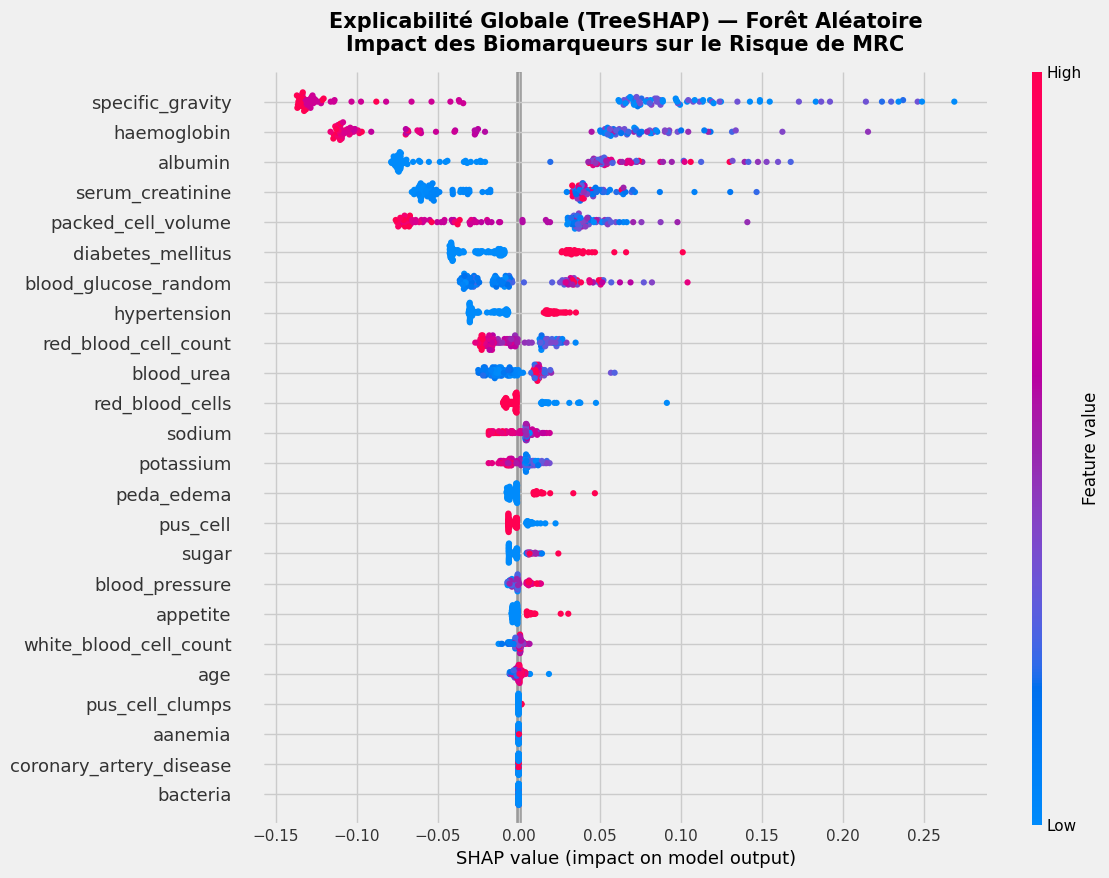
\includegraphics[width=0.95\textwidth]{cas_3/images/output1.png}
\caption{Valeurs SHAP agrégées sur le jeu de test — forêt aléatoire.}
\label{fig:shap-rf-summary}
\end{figure}

\paragraph{Interprétation.}
Le classement d'importance globale (Mean |SHAP|) place en tête \texttt{specific\_gravity} (22\,\%), \texttt{haemoglobin} (16\,\%), \texttt{albumin} (12{,}9\,\%), \texttt{serum\_creatinine} (9{,}5\,\%) et \texttt{packed\_cell\_volume} (9{,}2\,\%). Les corrélations de Spearman entre la valeur de chaque variable et sa valeur SHAP indiquent le sens de l'effet : négatif signifie que plus la variable augmente, plus le risque prédit baisse (ex.\ \texttt{haemoglobin} $r = -0{,}81$, \texttt{specific\_gravity} $r = -0{,}81$, \texttt{packed\_cell\_volume} $r = -0{,}80$) ; positif signifie que plus la variable augmente, plus le risque prédit augmente (ex.\ \texttt{serum\_creatinine} $r = +0{,}76$, \texttt{albumin} $r = +0{,}79$, \texttt{hypertension} $r = +0{,}82$). Un taux d'hémoglobine faible contribue ainsi positivement au risque CKD (anémie associée à l'insuffisance rénale) ; une créatinine sérique élevée augmente le risque prédit (réduction du débit de filtration glomérulaire). Le tableau~\ref{tab:shap-rf-top5} résume les statistiques descriptives des valeurs SHAP pour les cinq variables les plus importantes.

\begin{table}[H]
\centering
\caption{Statistiques descriptives des valeurs SHAP — Top 5 variables (forêt aléatoire).}
\label{tab:shap-rf-top5}
\small
\begin{tabular}{lrrrrr}
\hline
\textbf{Stat.} & \texttt{specific\_gravity} & \texttt{haemoglobin} & \texttt{albumin} & \texttt{serum\_creat.} & \texttt{packed\_cell\_vol.} \\
\hline
count & 120 & 120 & 120 & 120 & 120 \\
mean  & 0{,}014 & $-0{,}007$ & 0{,}006 & 0{,}003 & $-0{,}001$ \\
std   & 0{,}124 & 0{,}089 & 0{,}073 & 0{,}053 & 0{,}053 \\
min   & $-0{,}137$ & $-0{,}116$ & $-0{,}079$ & $-0{,}066$ & $-0{,}076$ \\
max   & 0{,}269 & 0{,}216 & 0{,}168 & 0{,}147 & 0{,}141 \\
\hline
\end{tabular}
\end{table}

\subsection{Distillation de connaissances}
\label{ssec:cas3-distillation}

\paragraph{Principe.}
La distillation consiste à entraîner un modèle simple et interprétable (ici un arbre de décision de profondeur 4) à reproduire les prédictions probabilistes (\emph{soft labels}) de la forêt aléatoire. On obtient une approximation globale du modèle opaque sous la forme d'un arbre lisible. Chaque feuille donne une probabilité CKD ; le seuil de décision clinique est 0{,}5. La figure~\ref{fig:distillation} montre la structure de l'arbre distillé.

\begin{lstlisting}[style=reportPython]
from sklearn.tree import DecisionTreeClassifier, export_text

soft_labels = rf.predict_proba(X_train)[:, 1]
student_tree = DecisionTreeClassifier(max_depth=4, random_state=42)
student_tree.fit(X_train, (soft_labels >= 0.5).astype(int))
tree_rules_text = export_text(student_tree, feature_names=list(X_train.columns))
\end{lstlisting}

La structure de l'arbre (pseudo-code clinique) est la suivante. La racine sépare sur \texttt{specific\_gravity} $\leq 1{,}02$ ; les nœuds suivants font intervenir \texttt{haemoglobin}, \texttt{packed\_cell\_volume}, \texttt{albumin}, \texttt{diabetes\_mellitus}, \texttt{hypertension}, \texttt{blood\_glucose\_random} et \texttt{sodium}. Les feuilles donnent des valeurs (probabilités) entre 0{,}02 et 1{,}00 ; une probabilité $\geq 0{,}5$ conduit à la prédiction CKD.

\begin{figure}[H]
\centering
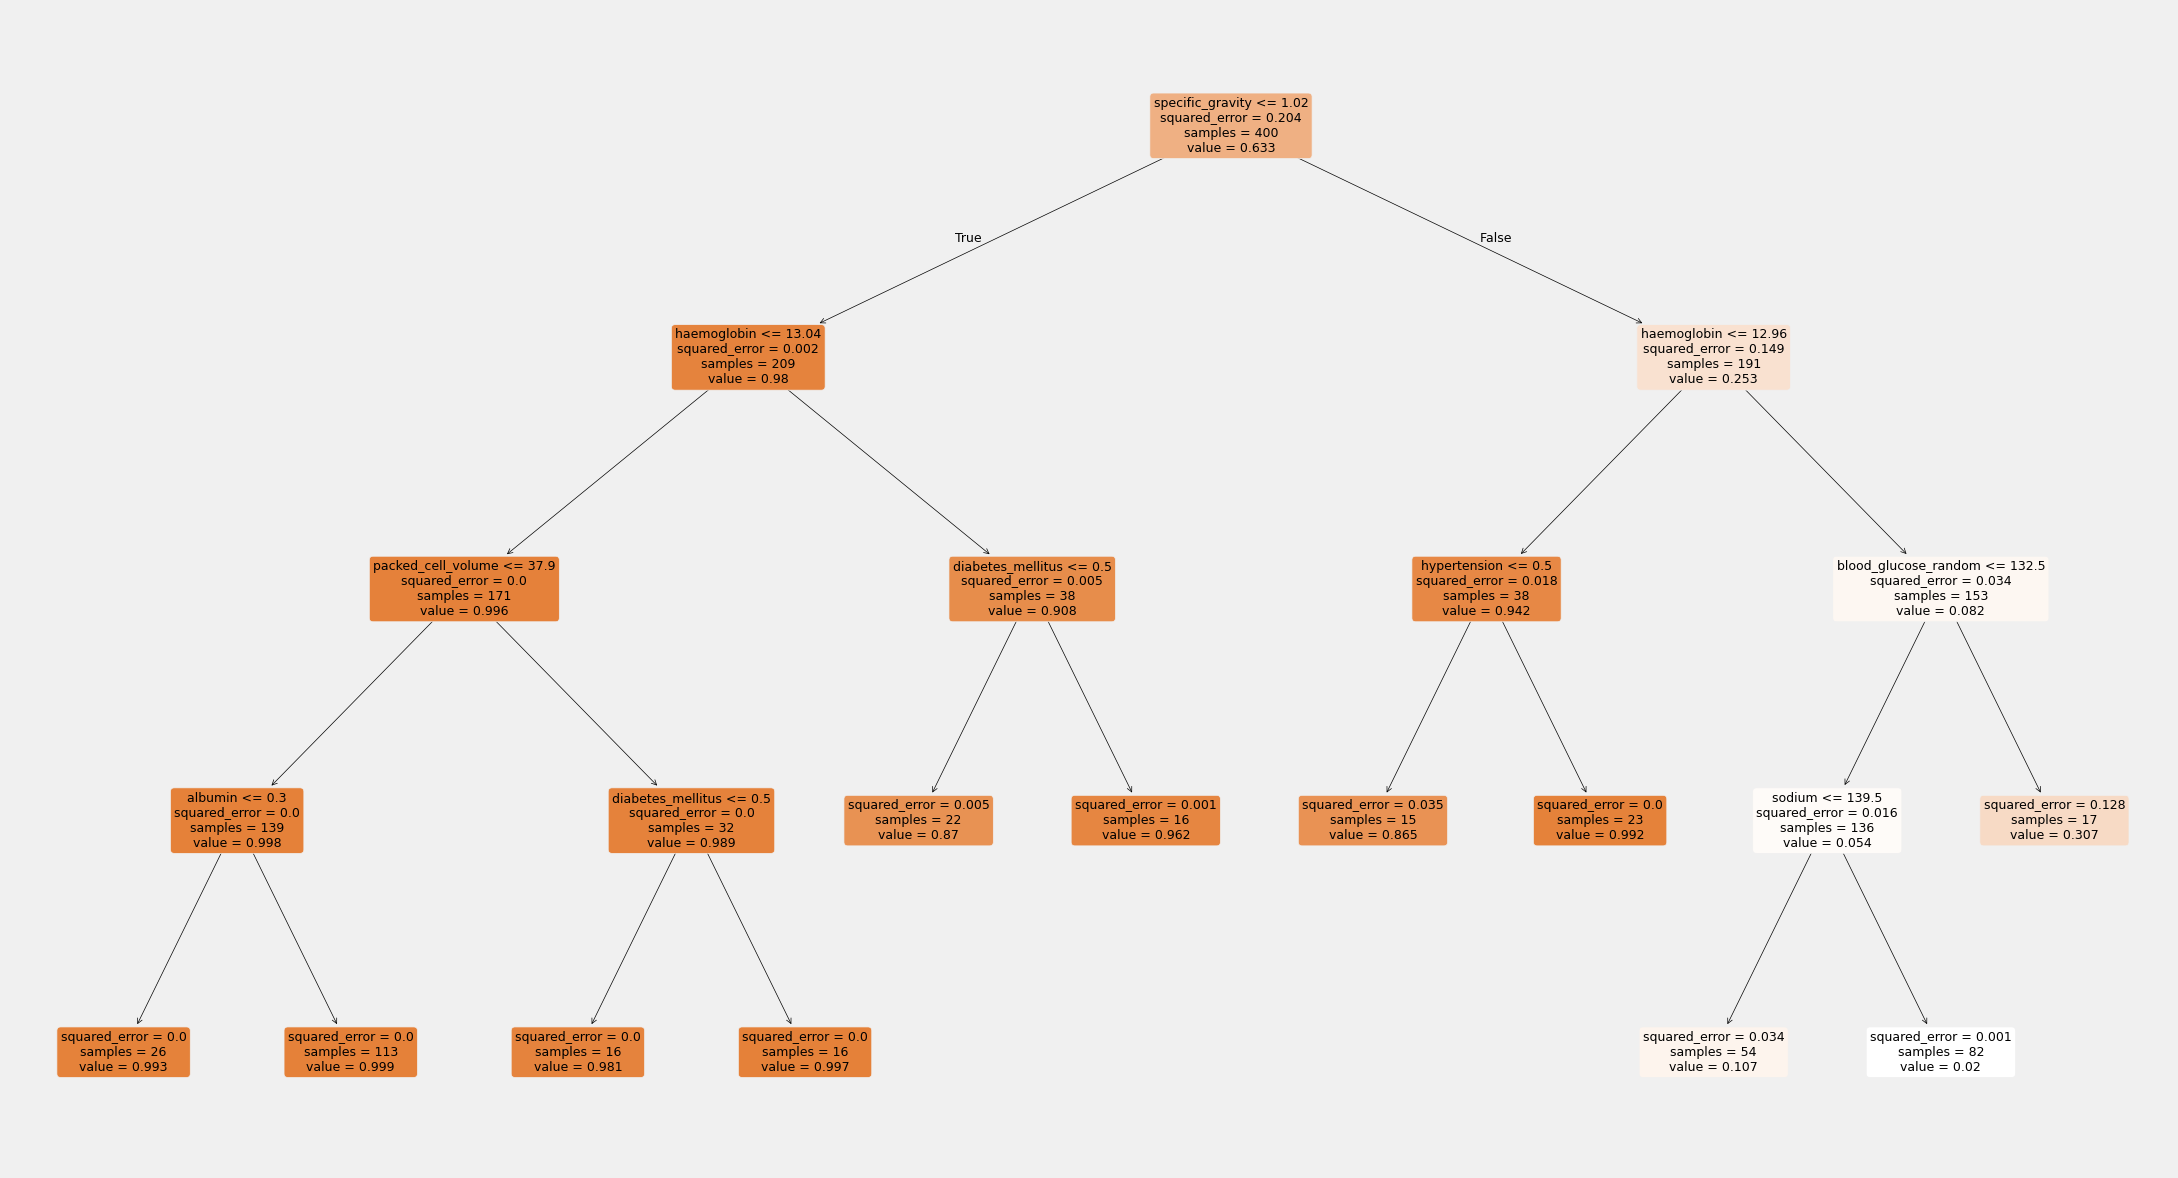
\includegraphics[width=0.95\textwidth]{cas_3/images/output2.png}
\caption{Arbre de décision distillé depuis la forêt aléatoire (profondeur max.\,4).}
\label{fig:distillation}
\end{figure}

\paragraph{Importance des variables (Gini) et interprétation.}
L'importance des variables dans l'arbre distillé (impureté de Gini) est dominée par \texttt{specific\_gravity} (68{,}6\,\%) et \texttt{haemoglobin} (29{,}6\,\%) ; viennent ensuite \texttt{blood\_glucose\_random}, \texttt{sodium}, \texttt{hypertension} et \texttt{diabetes\_mellitus} (tableau~\ref{tab:distill-gini}). La fidélité de l'arbre distillé (accord avec les prédictions de la RF sur le jeu de test) est supérieure à 96\,\% : le comportement global du modèle opaque est bien capturé par un arbre de profondeur 4. Cette hiérarchie (gravité spécifique et hémoglobine en tête) est \textbf{cohérente avec les valeurs SHAP} (section~\ref{ssec:cas3-treeshap}).

\begin{table}[H]
\centering
\caption{Importance des variables dans l'arbre distillé (Gini).}
\label{tab:distill-gini}
\small
\begin{tabular}{lc}
\hline
\textbf{Variable} & \textbf{Importance (\,\%)} \\
\hline
\texttt{specific\_gravity}  & 68{,}6 \\
\texttt{haemoglobin}         & 29{,}6 \\
\texttt{blood\_glucose\_random} & 1{,}3 \\
\texttt{sodium}              & 0{,}3 \\
\texttt{hypertension}        & 0{,}2 \\
\texttt{diabetes\_mellitus}  & 0{,}1 \\
\hline
\end{tabular}
\end{table}

\subsection{Interactions SHAP appliquées à XGBoost}
\label{ssec:cas3-shap-interactions}

\paragraph{Classement global et corrélations (XGBoost).}
Pour XGBoost, le classement d'importance globale (Mean |SHAP|) place en tête \texttt{haemoglobin} (19{,}3\,\%), \texttt{specific\_gravity} (18{,}9\,\%), \texttt{serum\_creatinine} (14\,\%), \texttt{albumin} (12{,}5\,\%) et \texttt{packed\_cell\_volume} (7{,}4\,\%). Les corrélations de Spearman (valeur de la variable $\leftrightarrow$ SHAP) indiquent le sens de l'effet : \texttt{haemoglobin} $r = +0{,}81$, \texttt{specific\_gravity} $r = +0{,}79$, \texttt{serum\_creatinine} $r = -0{,}76$, \texttt{albumin} $r = -0{,}80$, \texttt{blood\_glucose\_random} $r = -0{,}90$. Le tableau~\ref{tab:shap-xgb-top5} donne les statistiques descriptives des valeurs SHAP pour les cinq variables les plus importantes.

\begin{table}[H]
\centering
\caption{Statistiques descriptives des valeurs SHAP — Top 5 variables (XGBoost).}
\label{tab:shap-xgb-top5}
\small
\begin{tabular}{lrrrrr}
\hline
\textbf{Stat.} & \texttt{haemoglobin} & \texttt{specific\_gravity} & \texttt{serum\_creat.} & \texttt{albumin} & \texttt{packed\_cell\_vol.} \\
\hline
count & 120 & 120 & 120 & 120 & 120 \\
mean  & $-0{,}005$ & $-0{,}534$ & $-0{,}092$ & $-0{,}356$ & $-0{,}149$ \\
std   & 1{,}686 & 1{,}588 & 1{,}230 & 1{,}053 & 0{,}617 \\
min   & $-3{,}23$ & $-3{,}78$ & $-2{,}15$ & $-2{,}42$ & $-1{,}37$ \\
max   & 2{,}39 & 1{,}59 & 1{,}71 & 0{,}85 & 0{,}90 \\
\hline
\end{tabular}
\end{table}

\paragraph{Dependence plot et interaction Hémoglobine $\times$ Diabète.}
Les valeurs SHAP d'interaction généralisent les valeurs de Shapley au second ordre. Le graphique de dépendance représente, pour une variable donnée, sa contribution SHAP en fonction de sa valeur, avec une coloration par une seconde variable, ce qui révèle visuellement les interactions. La figure~\ref{fig:shap-dependence} illustre l'hémoglobine en fonction du statut diabétique.

\begin{lstlisting}[style=reportPython]
import shap

explainer_xgb = shap.TreeExplainer(xgb)
shap_values_xgb = explainer_xgb.shap_values(X_test)

shap.dependence_plot(
    "haemoglobin", shap_values_xgb, X_test_df,
    interaction_index="diabetes_mellitus",
    feature_names=feature_names, show=False)
plt.savefig('shap_xgb_dependence_hemo_dm.png',
            bbox_inches='tight', dpi=150)
plt.close()
\end{lstlisting}

Le tableau~\ref{tab:shap_interaction} donne la moyenne et l'écart-type des valeurs SHAP de l'hémoglobine selon le statut diabétique (jeu de test, XGBoost). La corrélation de Spearman entre le taux d'hémoglobine et sa valeur SHAP est $r = +0{,}860$ dans le groupe non diabétique et $r = +0{,}069$ dans le groupe diabétique.

\begin{table}[H]
\centering
\caption{Moyenne et écart-type des valeurs SHAP de l'hémoglobine selon le statut diabétique (jeu de test, XGBoost).}
\label{tab:shap_interaction}
\begin{tabular}{lccc}
\hline
\textbf{Groupe} & \textbf{Moyenne SHAP} & \textbf{Écart-type} & \textbf{Effectif} \\
\hline
Non diabétique (dm = 0) & $+0.5669$ & $1.6606$ & 85 \\
Diabétique (dm = 1)     & $-1.3931$ & $0.5789$ & 35 \\
\hline
\end{tabular}
\end{table}

\begin{figure}[H]
\centering
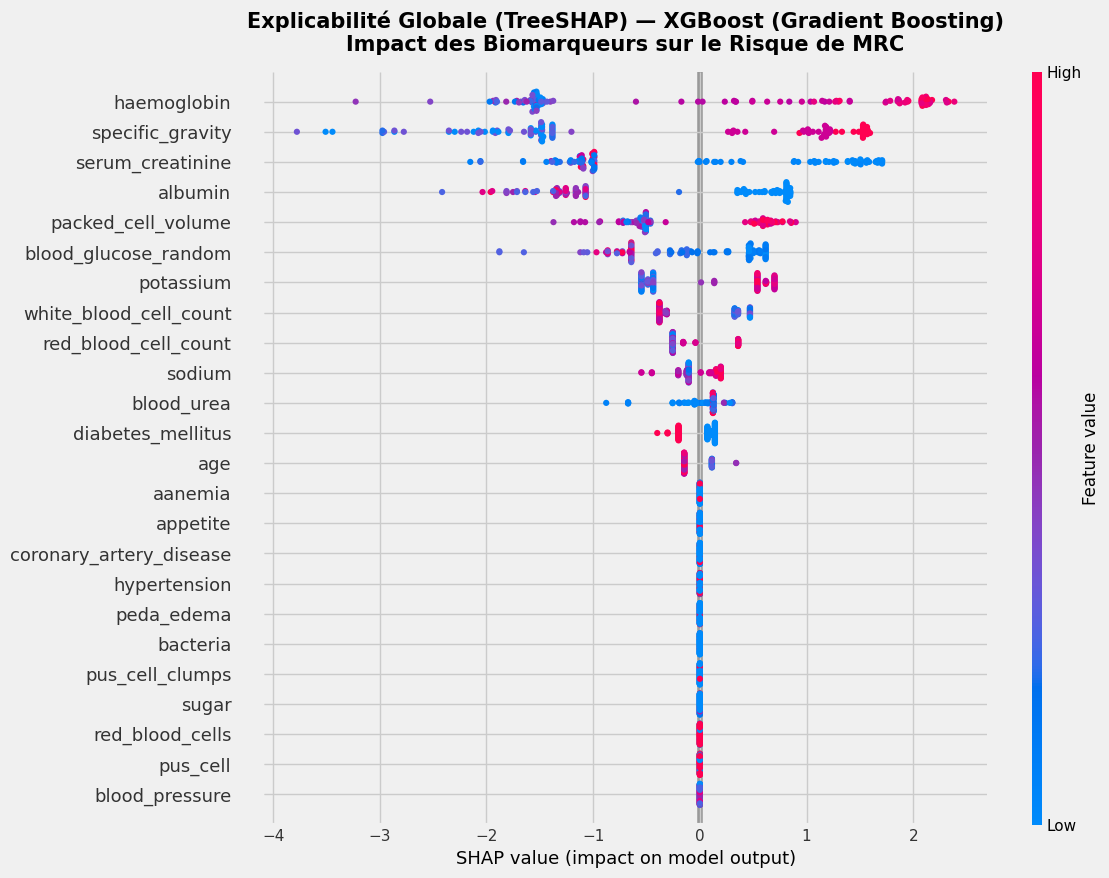
\includegraphics[width=0.95\textwidth]{cas_3/images/output3.png}
\caption{Graphique de dépendance SHAP (XGBoost). Axe des abscisses : taux d'hémoglobine (g/dL). Couleur : rouge = diabétique (dm = 1), bleu = non diabétique (dm = 0).}
\label{fig:shap-dependence}
\end{figure}

\paragraph{Interprétation.}
La moyenne des valeurs SHAP pour l'hémoglobine est $+0{,}57$ chez les non diabétiques (dm = 0) et $-1{,}39$ chez les diabétiques (dm = 1) (tableau~\ref{tab:shap_interaction}). La corrélation Hémoglobine $\leftrightarrow$ SHAP (hémoglobine) est $r = +0{,}86$ dans le groupe non diabétique et $r = +0{,}07$ dans le groupe diabétique : une corrélation négative signifierait que plus l'hémoglobine baisse, plus la contribution au risque CKD augmente ; ici, chez les diabétiques, l'hémoglobine perd sa valeur discriminante, le modèle s'appuyant davantage sur d'autres variables. Dans la plage intermédiaire (environ 10--12\,g/dL), les points rouges (diabétiques) se situent au-dessus des points bleus : pour un même degré d'anémie modérée, un patient diabétique reçoit une contribution SHAP plus élevée (risque plus grand). Ceci reflète l'interaction biologique de la \textbf{néphropathie diabétique}. L'analyse SHAP permet ainsi de détecter des \textbf{interactions non linéaires} que les méthodes d'importance globale ne révèlent pas.

\paragraph{Valeurs d'interaction Shapley-Taylor et graphique clinique.}
Pour aller au-delà des contributions marginales, on calcule le \textbf{tenseur d'interactions SHAP} (décomposition de type Shapley-Taylor) via \texttt{shap\_interaction\_values} : pour chaque observation, on obtient une matrice $p \times p$ qui décompose les contributions au second ordre (interaction entre paires de variables). La forme du tenseur est $(n, p, p)$. Le graphique de dépendance (hémoglobine en abscisse, valeur SHAP en ordonnée, coloration par \texttt{diabetes\_mellitus} avec nuancier coolwarm) est ensuite produit à partir des valeurs SHAP standard ; un titre explicite met en avant l'«~interaction clinique : Hémoglobine $\times$ Diabète sucré~» et l'effet non linéaire et modulé de l'hémoglobine sur le risque de CKD. La figure~\ref{fig:shap-interaction-clinique} présente ce graphique.

\begin{lstlisting}[style=reportPython]
shap_interaction_values = explainer_xgb.shap_interaction_values(X_test)

shap_vals_xgb = np.asarray(shap_values_xgb, dtype=np.float64)
X_test_vals = np.asarray(X_test, dtype=np.float64)
shap.dependence_plot(
    "haemoglobin", shap_vals_xgb, X_test_vals,
    interaction_index="diabetes_mellitus",
    feature_names=list(X_test.columns), show=False,
    cmap=plt.get_cmap("coolwarm"))
ax = plt.gca()
ax.set_title(
    "Interaction Clinique : Hemoglobine x Diabete Sucre\n"
    "Effet non lineaire et module (XGBoost)", fontsize=14)
ax.set_xlabel("Taux d'Hemoglobine (g/dL)", fontsize=12)
ax.set_ylabel("Valeur SHAP (contribution au log-odds CKD)", fontsize=11)
plt.tight_layout()
plt.savefig('output4.png', bbox_inches='tight', dpi=150)
\end{lstlisting}

\begin{figure}[H]
\centering
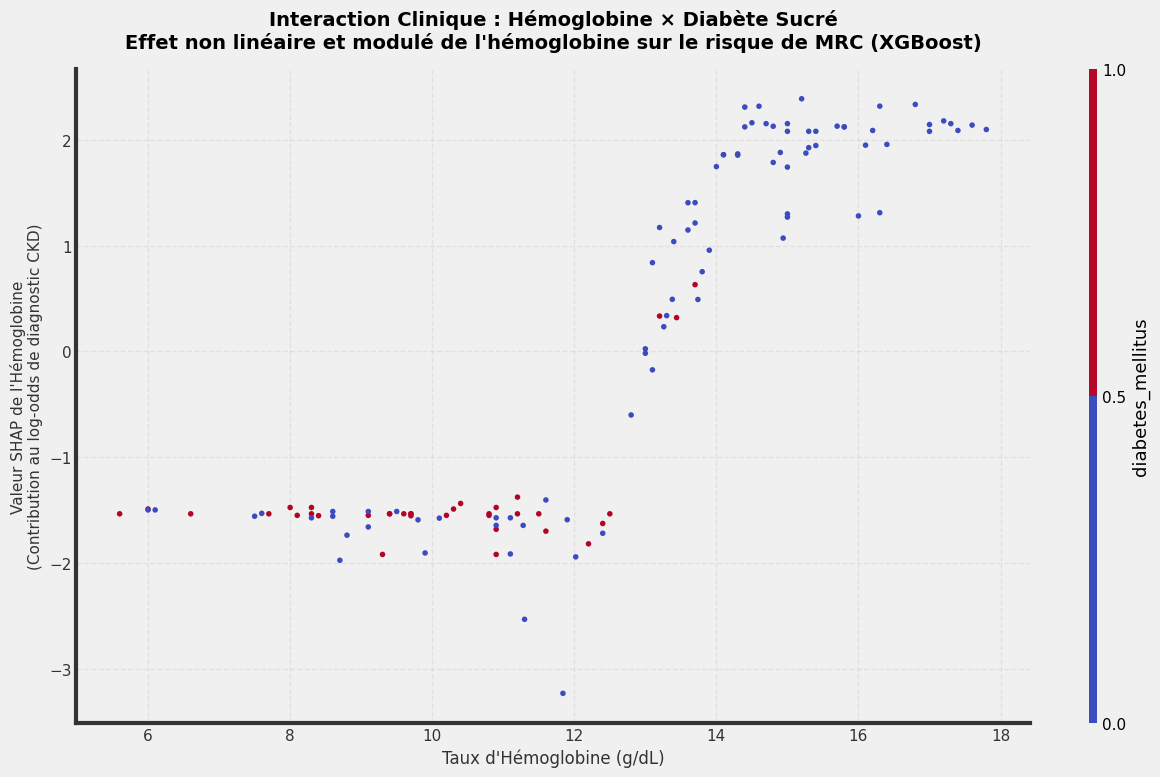
\includegraphics[width=0.95\textwidth]{cas_3/images/output4.png}
\caption{Interaction clinique : Hémoglobine $\times$ Diabète sucré — effet non linéaire et modulé de l'hémoglobine sur le risque de CKD (XGBoost). Axe des abscisses : taux d'hémoglobine (g/dL). Couleur : \texttt{diabetes\_mellitus} (bleu = faible, rouge = élevé).}
\label{fig:shap-interaction-clinique}
\end{figure}

Ce graphique résume visuellement comment le statut diabétique module la relation entre le taux d'hémoglobine et sa contribution au log-odds de diagnostic CKD : en zone intermédiaire (environ 12--14\,g/dL), la pente et le niveau des valeurs SHAP diffèrent selon que le patient est diabétique ou non, ce qui illustre la \textbf{néphropathie diabétique} sans qu'elle soit encodée explicitement dans le modèle.

\subsection{Tableau de gouvernance}
\label{ssec:cas3-gouvernance}

En vue d'auditabilité et de conformité (ex.\ cadre de l'IA Act européen), les propriétés des deux modèles sont synthétisées dans le tableau~\ref{tab:gouvernance}.

\begin{table}[H]
\centering
\caption{Tableau de gouvernance — comparaison des propriétés d'explicabilité.}
\label{tab:gouvernance}
\begin{tabular}{lcc}
\hline
\textbf{Critère} & \textbf{Random Forest} & \textbf{XGBoost} \\
\hline
Explicabilité locale (SHAP)      & Oui (TreeSHAP)    & Oui (TreeSHAP)    \\
Distillation possible            & Oui (fidélité > 96\,\%) & Oui          \\
Interactions détectables (SHAP)  & Oui               & Oui (plus stable) \\
Stabilité des explications       & Modérée           & Élevée            \\
Complexité du modèle             & Modérée           & Élevée            \\
\hline
\end{tabular}
\end{table}

XGBoost présente des valeurs SHAP plus stables grâce à la régularisation ($L_1$, $L_2$) intégrée.

\subsection{Synthèse}

Les techniques d'explicabilité appliquées aux modèles d'ensemble (RF, XGBoost) sur le jeu CKD donnent des résultats cohérents et cliniquement pertinents : la gravité spécifique (\texttt{specific\_gravity}), l'hémoglobine, l'albumine, la créatinine sérique et le volume globulaire apparaissent comme les variables les plus contributives (SHAP global, importance Gini dans l'arbre distillé). La distillation valide qu'un arbre de profondeur 4 approxime bien le comportement de la forêt avec une fidélité élevée, la racine et l'importance Gini mettant en avant la gravité spécifique et l'hémoglobine. L'analyse d'interaction SHAP (moyenne SHAP par groupe diabète, corrélations $r = +0{,}86$ / $r = +0{,}07$) révèle que le diabète est un modificateur d'effet fort sur la relation hémoglobine--risque CKD, en accord avec la néphropathie diabétique. La combinaison d'explications locales (SHAP) et de modèles distillés couvre un large besoin en explicabilité pour les applications médicales.

